% Tex root = ../cheatsheet.tex
\section{Gewöhnliche Differentialgleichungen (ODE)}
  \definition{2.1.0.1}{ODE}
  Sei $k\geq1$, $U\subseteq\mathbb R^{k+2}$, $G:U\rightarrow\mathbb R$. Dann ist 
  $$G(x,y,y',y'',...,y^{(k)})=0$$ eine ODE $k$-ter Ordnung.\\
  \definition{2.1.0.2}{Lösung einer ODE}
  Eine Lösung einer ODE der Ordnung $k$ ist eine $k$-mal diffbare Funktion $f:I\rightarrow\mathbb R$
  auf einem offenen Intervall $I\subseteq\mathbb R$ mit $$G(x, f(x). f'(x),...,
  f^{(k)}(x))=0$$.\\
  \definition{2.1.0.3}{Anfangswertproblem (AWP)}
  Sind bei einer ODE zusäzlich noch Anfangsbedinungen gegeben, d.h.
  $$y(x_0)=y_0,y'(x_0)=y_1,...,y^{(k-1)}(x_0)=y_k$$ mit $x_0,
  y_0,...,y_k\in\mathbb R$, dann liegt ein AWP vor.\\
  \rmrk{2.1.0.4}{} k wird generell minimal angegeben. \\
  $G(x, y)=0$ ist \textbf{keine} ODE.\\
  Lässt sich eine ODE als $y^{(k)}=F(x,y,y',...,y^{(k-1)})$ schreiben so nennen
  wir diese \textbf{explizit}.\\
  Stammfunktionsprobleme sind Spezialfälle einer ODE, z.B. $y'=1/x$.\\
  Sind ODEs nicht von $x$ abhängig so nennt man diese \textbf{Autonom}. Beispielsweise
  $y''=1/m$\\
\subsection{Einführung}
  \proposition{2.1.6}{Existenz- und Eindeutigkeitssatz}
  Ein AWP $y'=F(x,y)$, $y(x_0)=y_0$ mit $F:\ U\rightarrow\mathbb R$ stetig für
  $U\in\mathbb R^2$ offen, $(x_0,y_0)\in U$, hat eine Lösung.\\
  Ist $F$ stetig differenzierbar, so gibt es eine \textbf{eindeutige maximale}
  Lösung. (Maximal bedeutet, es ist nicht eine Einschränkung einer anderen Lösung
  mit grösserem Intervall.)\\
  \definition{2.1.7}{Vektorfelddarstellung}
  Eine Explizite ODE der Form $y'=F(x,y)$ mit $F: U\subseteq\mathbb 
  R^2\rightarrow\mathbb R$ lässt sich durch das Vektorfeld $V: 
  U\rightarrow\mathbb R^2, V(x,y) = (1, F(x,y))$ visualisieren. Eine Lösung $f: 
  I\rightarrow\mathbb R$ des ODE hat als Graph eine Kurve beschrieben durch
  $\phi:I\rightarrow\mathbb R^2, \phi(x)=(x,f(x))$ mit $\phi'(x)=(1,
  f'(x))=V(x,y)$. D.h. $\phi$ ist an jedem Punkt tangential zum Vektorfeld V.\\
  \begin{minipage}{\linewidth}
    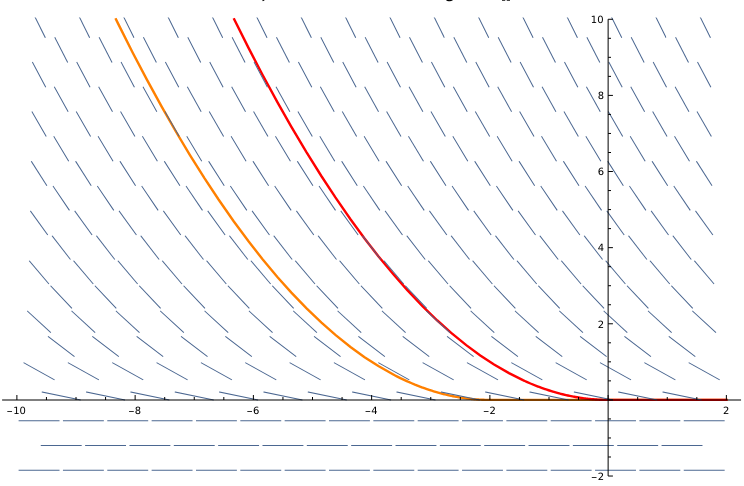
\includegraphics[width=\linewidth]{./sources/beispiel_vektorfelddarstellung.png}
  \end{minipage}
\subsection{Lineare ODE}
  \definition{2.2.1}{Lineare ODE}
  Eine Lineare ODE ist eine ODE von Ordnung $k\geq1$ der Form
  $$y^{(k)}+a_{k-1}y^{(k-1)}+...+a_0y=b$$ Koeffizienten $a_{k-1},...,a_0$ und
  inhomogenität $b$ sind Funktionen $I\rightarrow\mathbb C$ für ein offenes
  Intervall $I\in\mathbb R$.
  Falls $b=0$, heisst die lineare ODE \textbf{homogen}, sonst
  \textbf{inhomogen}. Falls wir eine inhomogene lineare ODE haben, ist die
  \textbf{zugehörige homogene lineare ODE}: $$y^{(k)}+...+a_0y=0$$
  Eine Lösung ist eine k-mal differenzierbare $f:I\rightarrow \mathbb C$
  $$f^{(k)}(x)+...+a_0(x)f(x)=b(x)\hspace{1cm}\forall x\in\mathbb R$$ wobei
  $f^{(j)}=(Re\; f(x))^{(j)} + i \cdot(Im\; f(x))^{(j)}$\\
  \definition{2.2.5}{Superpositionsprinzip}
  $$\begin{array}{rll}
    f_0&\text{Lösung der ODE mit inhomogenität}&b\\
    g_0&\text{Lösung der ODE mit inhomogenität}&c\\
    \lambda f_0+\mu g_0&\text{Lösung der ODE mit inhomogenität}&\lambda b +\mu
    c.
  \end{array}$$
  \definition{2.2.8}{}
  Für eine lineare ODE $(1)$ $k$-ter Ordnung mit stetigen $a_{k-1},...,a_0,b$ gilt:\\
  $*$ Die Lösungen der zugehörigen homogenen ODE $(2)$ bilden einen $\mathbb 
  C$-Vektorraum $S$ mit $\dim_{\mathbb C}S=k$\\
  $*$ Die inhomogene ODE (1) hat eine Lösung $f_0$. Die Menge aller Lösungen
  bildet dann den affinen Raum $$f_0+S=\{f_0+f\mid f\in S\}$$\\
  $*$ Für beliebige $x_0\in I$ und $y_0,...,y_{k-1}\in\mathbb C$ hat das
  dazugehörige AWP (1) genau eine Lösung.\\\\
  Sind $a_{k-1},...,a_0,b$ reellwertig, dann gilt:\\
  $*$ Reelwertige Lösungen der zugehörigen homogenen ODE (2) bilden einen
  $\mathbb R$-Untervektorraum $S_{\mathbb R}$ von $S$ mit $dim_{\mathbb R}=k$\\
  $*$ Die inhomogene ODE (1) hat eine reelwertige Lösung $f_0$ und die Menge
  aller Lösungen bildet den affinen $\mathbb R$-Raum $$f_0+S_{\mathbb R}$$\\
  $*$ Für $y_0,...,y_{k-1}\in\mathbb R$ hat das zugehörige AWP genau eine
  reelwertige Lösung.\\
  \example{2.2.8.1}{Lösungsstrategie für Lineare ODEs}
  \begin{enumerate}
    \item Finde eine Basis \(f_1,...,f_k\) des Lösungsraums \(S\) der homogenen ODE\\
      \color{Maroon3} \(k=1\): finde eine Lösung \(f_1\neq0\).\color{defaultcolor}
    \item Finde eine einzelne Lösung $f_0$ der inhomogenen ODE (Partikulärlösung).
      Allg. Lösung: \(f_0+\sum\limits_{i=1}^{k}\lambda_i f_i\).\\
      \color{Maroon3} \(k=1\): allg. Lösung \(f_0+\lambda
      f_1\)\color{defaultcolor}
    \item Einsetzen der Anfangswerte \(\rightsquigarrow\) lineares
      Gleichungssystem für \(\lambda_1,...,\lambda_k\) mit eindeutiger Lösung.\\
      \color{Maroon3}\(k=1\): \(f_0(x_0)+\lambda f_1(x_0) = y_0 \implies \lambda
      = \frac{y_0 - f(x_0)}{f_1(x_0}\)
  \end{enumerate}
\subsection{Lineare ODE erster Ordnung}
  Zu lösen: $y'+ay=b$ mit gegebenen stetigen $a,b: I \rightarrow\mathbb C$\\
  \proposition{2.3.1}{Die Lösungen der ODE} Die Lösungen für die homogene ODE $$y'+ay=0$$ sind genau die
  Funktionen $ze^{-A(x)}$ für $z\in\mathbb C$ und A eine Stammfunktion von a.\\
  Für die inhomogene ODE $$y'+ay=b$$ Ansatz $f(x)=z(x)\cdot e^{-A(x)}$.
  Einsetzen in die ODE gibt uns $f'+af=b$\\
  \indent $\iff z'e^{-A}+zae^{-A}-aze^{-A}=b$\\
  \indent $\iff z'e^{-A}=b$\\
  \indent $\iff z'= e^{A}b$\\
  \indent $\iff z$ ist Stammfunktion von $e^{A}b$
\subsection{Lineare ODEs mit konstanten Koeffizienten}
  $$y^{(k)},a_{k-1}y^{(k-1)},...,a_0y=b$$ für $a_{k-1},...,a_0\in\mathbb C$ und
  $b:I\rightarrow\mathbb C$.\\
  \subsubsection{Homogene ODE}
    \definition{2.4.0.1}{Charakteristisches Polynom}
      $$P(t)=t^k+a_{k-1}t^{k-1}+...+a_0$$
      Ist das Charakteristische Polynom der linearen ODE.
    \proposition{2.4.0.2}{Lösen der homogenen ODE}
      \begin{enumerate}
        \item $P(\alpha)=0$ für $\alpha\in\mathbb C\implies e^{\alpha x}$ löst die
          homogene ODE.
        \item Hat $P$ keine mehrfachen Nullstellen, so ist $\{e^{\alpha x}\mid
          P(\alpha)=0\}$ eine Lösungsbasis.
      \end{enumerate}
    \proposition{2.4.0.3}{Basis des Lösungsraums}
      Hat $P$ die Nullstellen $\alpha_1,...,\alpha_l$ mit Vielfachheit
      $v_1,...,v_l$, so ist bildet die Menge $$\{x^je^{\alpha_i x}\mid 1\leq i<l,
      0\leq j<v_{i-1}\}$$ eine Bases des Lösungsraums.\\
    \rmrk{2.4.0.3}{}
      Falls $a_0,...,a_{k-1}\in\mathbb R$, dann gilt: $$P(\alpha)=0\iff
      P(\overline\alpha)=0$$ Man findet eine Basis des reelwertigen Lösungsraum,
      indem man $e^{\alpha x}, e^{\overline\alpha x}$ ersetzt durch $$e^{\beta
      x}\cos(\gamma x),e^{\beta x}\sin(\gamma x)$$ für $\alpha=\beta + i\gamma$.
  \subsubsection{Inhomogene ODE}
    \definition{2.4.1}{Methode der unbestimmten Koeffizienten}
    Wir schauen uns dafür die Form der Inhomogenität an:
    \begin{enumerate}
      \item[$*$] $b(x)=x^de^{\alpha x}$\hfill (Spezialfälle: $b=x^d$, 
        $b=e^{\alpha x}$)\\
        $\implies$ es gibt eine Lösung $f_0(x)=Q(x)e^{\alpha x}$, für ein
        Polynom $Q$ mit $\deg Q\leq d+j$, wobei $\alpha$ $j$-fache Nullstelle von
        $P$ (falls $P(\alpha)\neq0 \iff j=0$)
      \item[$*$] $b(x)=x^d\cos(\alpha x)$ oder $x^d\sin(\alpha x)$\\
        $\implies$ es gibt eine Lösung $f_0(x)=Q_1(x)\cos(\alpha
        x)+Q_2\sin(\alpha x)$, für Polynome $Q_1,Q_2$ mit Grad jeweils
        $\deg(Q_i) \leq d+j$, falls $\alpha_i$ $j$-fache Nullstelle von $P$
    \end{enumerate}
    Anleitung:
    \begin{enumerate}
      \item Benutze das Superpositionsprinzip (2.2.5) um die inhomogenität so 
        aufzuteilen, dass sie auf die oben genannten gleichungen passen.
      \item Finde die passende Funktion $f_0$ indem du $\alpha$ aus der (teil) inhomogenität
        abliest und in die vorgegebene Funktion einsetzt.
      \item Setze $f_0$ für $y$ in die ODE ein bzw die jeweiligen ableitungen.
      \item Finde die $Q_i$ für welche die Gleichung für alle $x$ gilt mit hilfe
        des Koeffizientenvergleichs.
            (Die $Q_i$ sind jeweils von der Form
        $q_0x^{i}+q_1x^{i-1}+...+q_i$ wobei $i=\deg Q$)
      \item Setze die $Q_i$ in $f_0$ ein um eine Lösung zu erhalten.
      \item Berechne die lösung der ursprungs ODE indem du die resultate der
        Teilhomogenitäten nach dem Superpositionsprinzip wieder
        zusammenrechnest.
    \end{enumerate}
\subsection{Other Methods}
  \definition{2.6.1}{Separation der Variablen}
  Für ODEs der Form $y'=a(y)\cdot b(x)$ und $a,b$ stetig.
  Für jede Nullstelle $y_0\in\mathbb R$ von $a$ gibt es eine Konstante Lösung
  $y(x)=y_0$.\\
  Für $a(y)\neq0$: ODE$\iff \frac{y'}{a(y)}=b(x)$\\
  $\iff\int \frac{y'}{a(y)}dx=\int b(x)dx+c$ für $c\in\mathbb R$
  \begin{enumerate}
    \item Finde Stammfunktion A,B von $\frac{1}{a}, b$\\
    $*$ Kettenregel: $\int\frac{y'}{a(y)}dx = A(y)+c$\\
    $\implies A(y)=B(x) + c$
    \item Falls A eine Umkehrfunktion hat, dann ist $y=A^{-1}(B(x)+x)$
  \end{enumerate}

